\documentclass[11pt]{article}
\usepackage[margin=0.72in]{geometry}
\usepackage{booktabs}
\usepackage{longtable}
\usepackage{graphicx}
\usepackage{xcolor}
\usepackage{hyperref}
\usepackage{array}
\hypersetup{colorlinks=true, linkcolor=blue, urlcolor=blue}
\setlength{\parindent}{0pt}
\setlength{\parskip}{6pt}

\title{Professor Meeting Script: Archive-2 SPY Call Options EDA}
\author{ML-Based Trading of TP2-Inspired Violations in SPY Call Options}
\date{Prepared for weekly project update}

\begin{document}
\maketitle

\section*{Purpose of This Update}

\textbf{What I would say:}

The goal of this update is to show that we have moved from the earlier smaller
sample to the professor-provided Archive-2 dataset, and that we now understand
the raw data well enough to start rebuilding the research pipeline carefully.
This is still the EDA and detector-validation stage, not the final ML trading
result.

The main result is: the dataset is broad enough for the project, but the raw
data must be handled transparently because it contains multiple quote
observations per contract-day, missing/skipped sessions, and quote-time
variation. We reconstructed an active clean dataset using the latest available
quote per SPY call contract-day, then ran the full forward-adjusted TP2
detector on it.

\section*{Raw Data Coverage}

\textbf{What I would say:}

The raw Archive-2 dataset covers SPY options from April 1, 2013 to June 4,
2026. The raw parquet files contain about 58.8 million observed rows across
3,256 trading sessions. One raw row is an option quote observation, not
necessarily one final end-of-day contract quote. Many contract-days appear more
than once in the raw files, so ingestion must collapse the raw observations to
one quote per contract-day before any TP2 detection.

\begin{center}
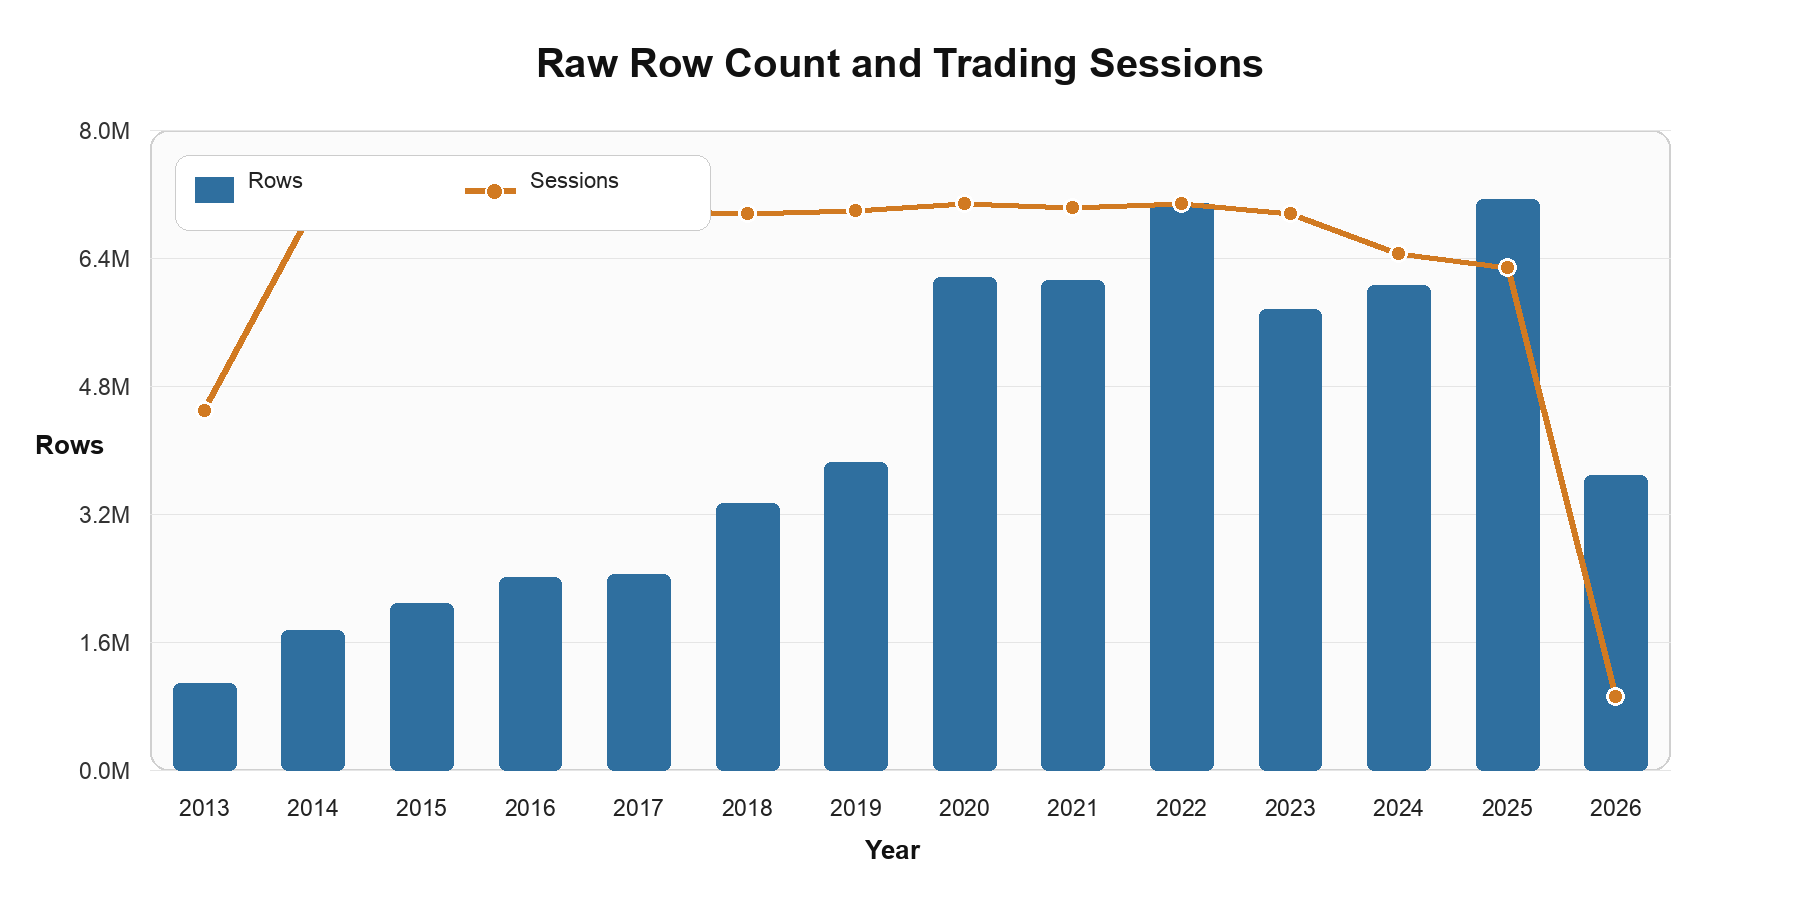
\includegraphics[width=0.96\textwidth]{raw_archive2_eda/figures/raw_rows_sessions_by_year.png}
\end{center}

\textbf{Key interpretation:} raw data volume grows over time, but higher raw
volume does not automatically mean more arbitrage opportunities. The TP2
detector forms many four-contract rectangles from the cleaned option chains,
and only a small subset of those rectangles violate the inequality.

\section*{Option Chain Breadth}

\textbf{What I would say:}

The option chain becomes broader over the sample period. Later years generally
have more contracts, strikes, and expirations per day. This matters because a
broader chain gives the detector more possible four-leg rectangles to compare.
For that reason, we should not compare yearly violation counts without also
showing the size of the clean quote universe.

\begin{center}
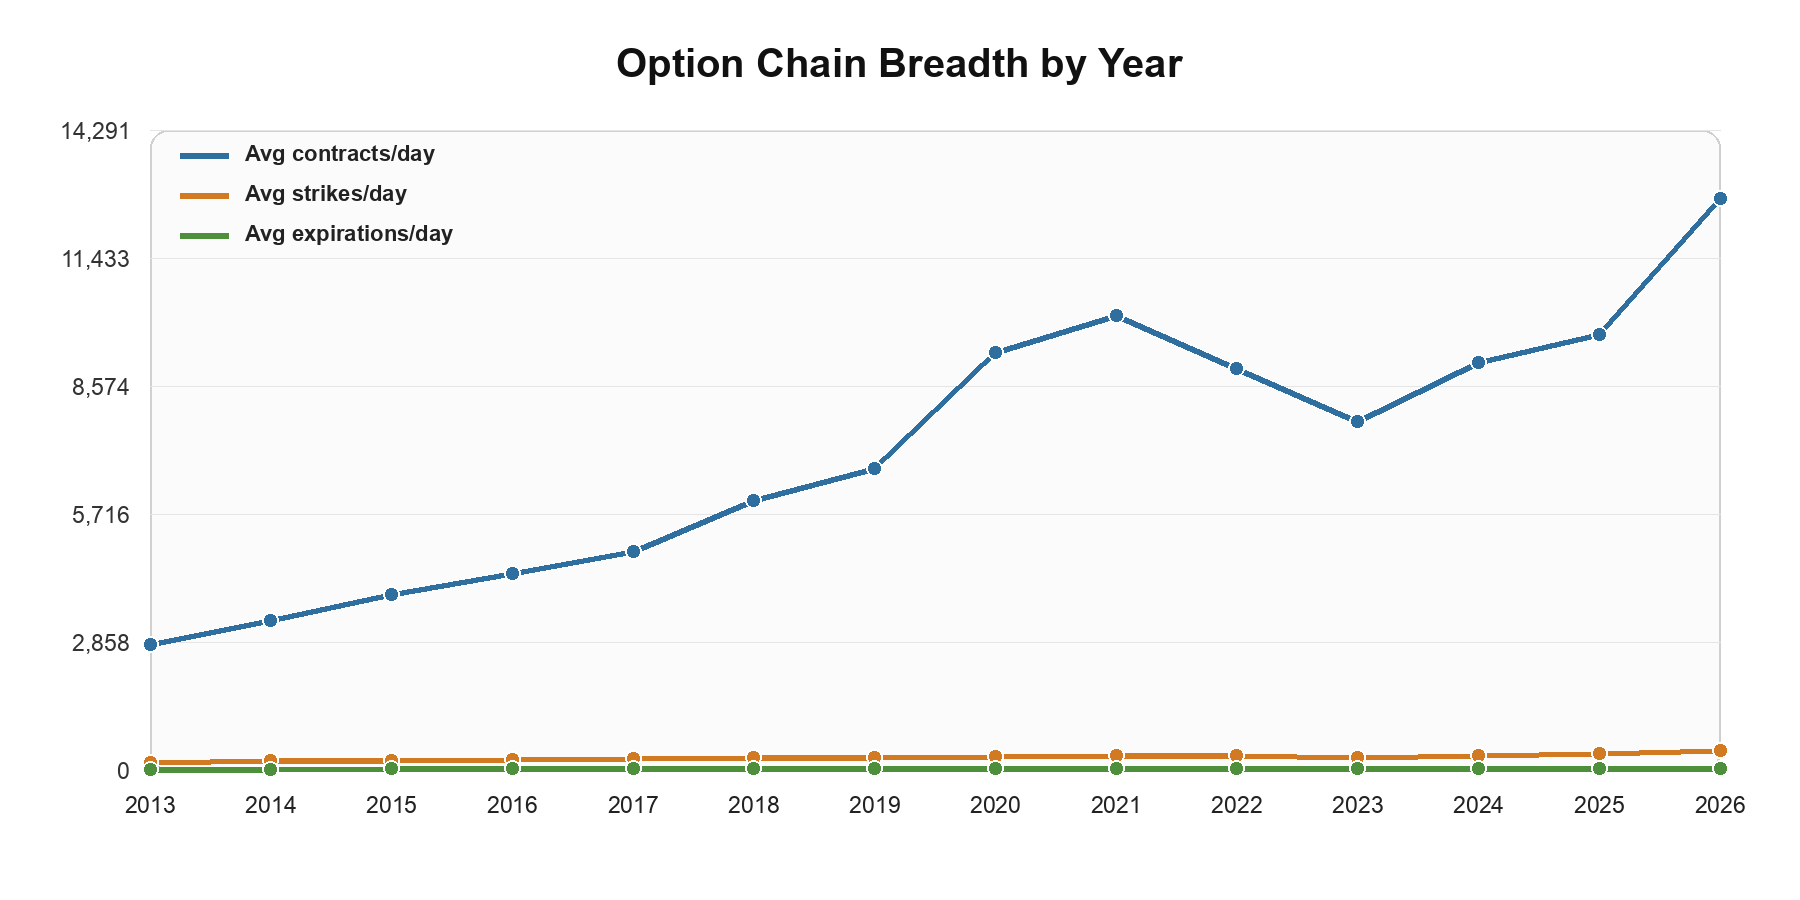
\includegraphics[width=0.96\textwidth]{raw_archive2_eda/figures/raw_chain_breadth_by_year.png}
\end{center}

\section*{Cleaning Decision}

\textbf{What I would say:}

Initially, we considered using only quotes after 15:55. After checking the raw
quote-time distribution, we found that the vendor data often stores the latest
available quote for the contract-day even when the timestamp is before 15:55.
Using a hard 15:55 cutoff removed too much otherwise usable data. Therefore,
the active clean dataset now uses the latest available quote per contract-day,
while keeping the same pricing-quality filters.

\begin{center}
\begin{tabular}{lrrrr}
\toprule
Dataset version & Rows & Sessions & Min DTE & Max DTE \\
\midrule
Old near-close $\geq$ 15:55 & 804,809 & 3,255 & 1 & 90 \\
New latest-available quote & 4,912,891 & 3,256 & 1 & 90 \\
\bottomrule
\end{tabular}
\end{center}

\textbf{Filters used in the active clean dataset:}
SPY calls only, DTE 1--90, valid bid/ask, positive bid, positive mid, and
spread percentage no greater than 50\%. The raw professor data was not modified;
the clean file is a separate derived research dataset.

\section*{TP2 Inequality Being Tested}

\textbf{What I would say:}

For calls, we are using the forward-adjusted TP2 condition from the
Glasserman--Li--Pirjol framework as the theoretical base. For $T_1<T_2$ and
$K_1/F_{T_1}<K_2/F_{T_2}$, the no-violation condition is:

\[
C(K_1,T_1)C(K_2,T_2)
\geq
C(K_1F_{T_2}/F_{T_1},T_2)C(K_2F_{T_1}/F_{T_2},T_1).
\]

The call violation condition is therefore:

\[
\mathrm{LHS}<\mathrm{RHS}.
\]

In the code, one detected violation row is one four-contract TP2 rectangle on
one quote date. It is not one option contract and not one executed trade.

\section*{What a ``Violation Row'' Means}

\textbf{What I would say:}

This is the most important interpretation point. A clean row is one usable
option quote, such as one SPY call contract on one date. A violation row is a
four-leg rectangle:

\[
A=C(K_1,T_1), \quad B=C(K_2,T_2), \quad
C=C(K_1F_{T_2}/F_{T_1},T_2), \quad
D=C(K_2F_{T_1}/F_{T_2},T_1).
\]

If $A_{\mathrm{mid}}B_{\mathrm{mid}} < C_{\mathrm{mid}}D_{\mathrm{mid}}$, that
four-leg rectangle becomes one TP2 violation row.

\textbf{2013 example:}

\begin{center}
\begin{tabular}{lr}
\toprule
Step & Count \\
\midrule
Clean individual option quote rows & 99,129 \\
Raw $K_1,K_2$ strike pairs across expiration pairs & 17,847,362 \\
After forward-order condition & 8,470,629 \\
Valid four-leg TP2 rectangles & 6,886,206 \\
TP2 violation rows after severity threshold & 73,619 \\
\bottomrule
\end{tabular}
\end{center}

So in 2013, about 6.89 million valid four-leg rectangles were possible from
99,129 clean option quotes, and about 1.07\% of those rectangles violated the
TP2 inequality.

\section*{Yearly TP2 Violation Counts}

\textbf{What I would say:}

The full detector found 2,430,220 daily TP2 violation rows across 2013--2026.
The detector output passed basic validation: zero rows had the wrong inequality
direction, zero rows had invalid expiration ordering, and zero duplicate
violation IDs were found across the yearly outputs.

\begin{center}
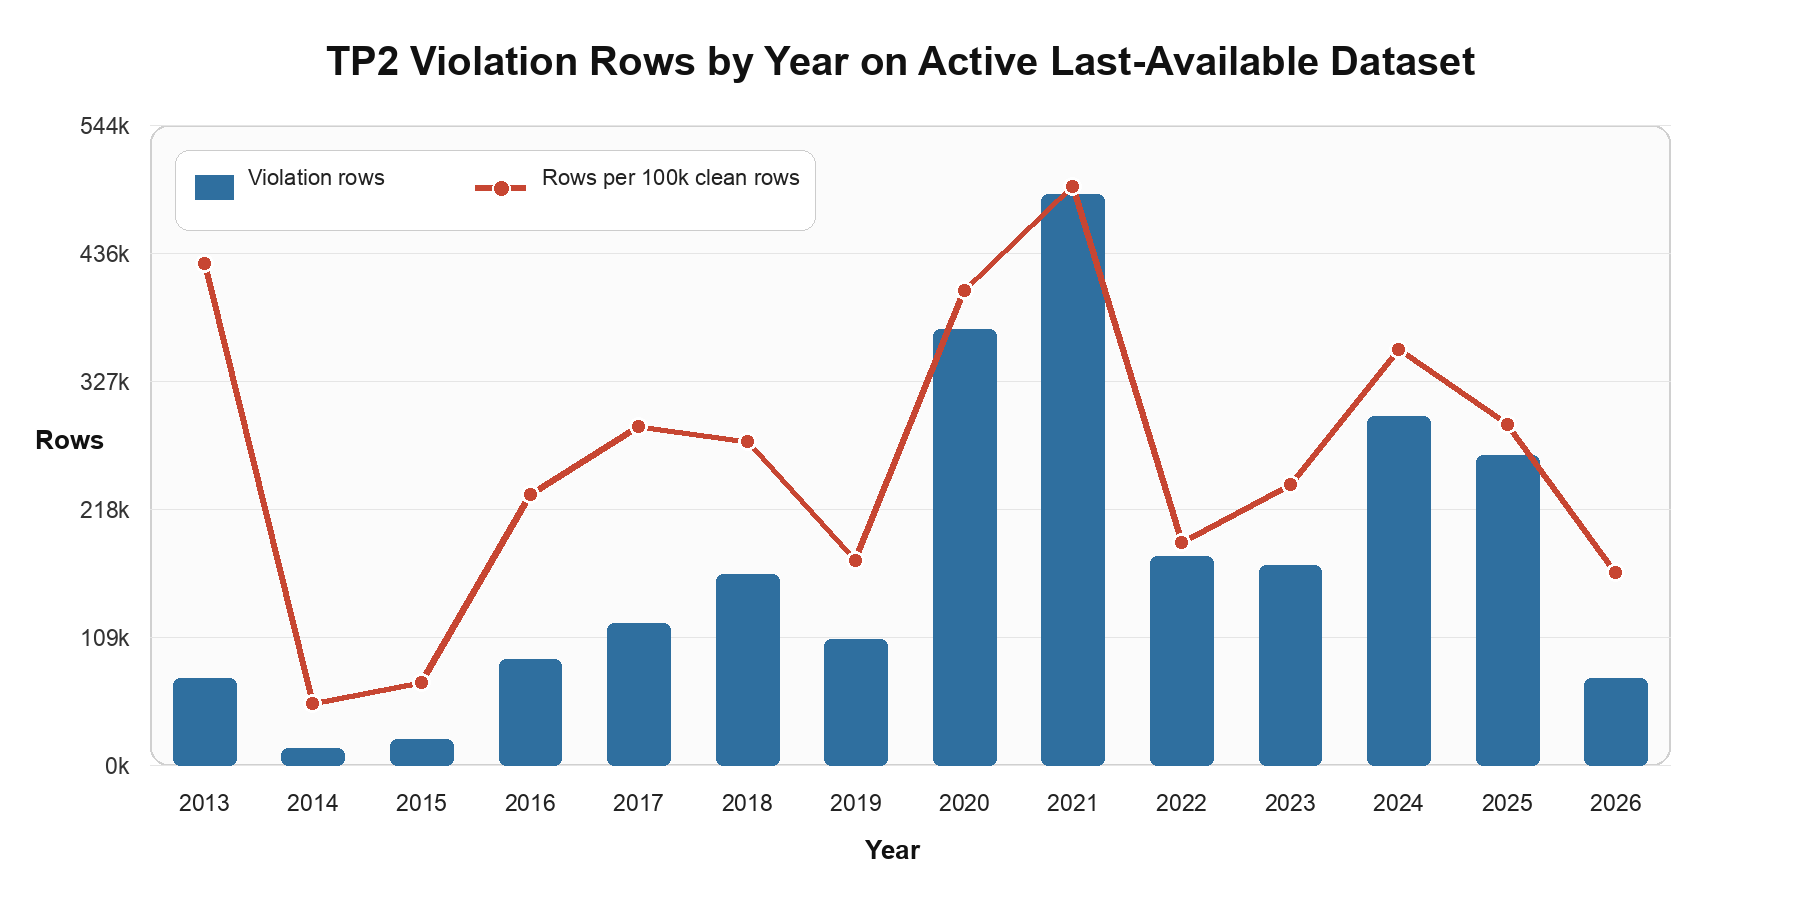
\includegraphics[width=0.96\textwidth]{raw_archive2_eda/figures/lastquote_tp2_violations_by_year.png}
\end{center}

\begin{center}
\scriptsize
\begin{tabular}{rrrrrr}
\toprule
Year & Clean rows & Sessions & Violation rows & Rows/session & Rows/100k clean \\
\midrule
2013 & 99,129 & 189 & 73,619 & 389.5 & 74,266 \\
2014 & 156,479 & 249 & 14,161 & 56.9 & 9,050 \\
2015 & 181,555 & 250 & 22,101 & 88.4 & 12,173 \\
2016 & 225,307 & 251 & 90,011 & 358.6 & 39,950 \\
2017 & 242,041 & 249 & 121,186 & 486.7 & 50,068 \\
2018 & 340,904 & 248 & 162,873 & 656.7 & 47,777 \\
2019 & 355,517 & 249 & 107,568 & 432.0 & 30,257 \\
2020 & 528,083 & 251 & 370,574 & 1,476.4 & 70,173 \\
2021 & 567,934 & 250 & 486,076 & 1,944.3 & 85,587 \\
2022 & 539,482 & 251 & 177,497 & 707.2 & 32,901 \\
2023 & 410,310 & 248 & 169,882 & 685.0 & 41,403 \\
2024 & 483,658 & 236 & 297,226 & 1,259.4 & 61,454 \\
2025 & 523,904 & 232 & 263,803 & 1,137.1 & 50,353 \\
2026 & 258,588 & 103 & 73,643 & 715.0 & 28,479 \\
\bottomrule
\end{tabular}
\end{center}

\textbf{How I would explain the columns:}
Clean rows are individual usable option quotes. Sessions are trading days.
Violation rows are four-contract TP2 rectangles that failed the inequality.
Rows/session is average violation rectangles per trading day. Rows/100k clean
normalizes violations by the amount of clean option quote data in that year.

\section*{Year-by-Year Rise and Dip Interpretation}

\textbf{What I would say:}

The yearly pattern should be interpreted as a detector-level EDA result, not
yet as a profitability result. A rise means the cleaned option surface produced
more TP2-violating four-leg rectangles. A dip means fewer such rectangles
passed the inequality and severity threshold. These movements can be driven by
market regime, option-chain breadth, quote quality, volatility, and repeated
same-rectangle violations across days.

\begin{center}
\scriptsize
\begin{tabular}{p{0.12\textwidth}p{0.22\textwidth}p{0.54\textwidth}}
\toprule
Year & Pattern & Interpretation for meeting discussion \\
\midrule
2013 & High relative to data size &
The year has only 189 sessions and fewer clean rows, but several months are
very concentrated. August, November, and December explain most of the annual
count. This suggests regime concentration rather than uniformly high activity. \\

2014 & Large dip &
Clean rows increase, but violation density falls sharply. This means more
option quotes did not translate into more TP2 failures. The surface appears
more internally consistent under our detector, or fewer rectangles crossed the
severity threshold. \\

2015 & Mild recovery &
Violation rows rise from 2014 but remain low compared with 2013. The increase
is modest and spread across more sessions, so this looks like a partial return
of violations rather than a concentrated spike. \\

2016 & Strong rise &
Clean rows and chain breadth increase, and the detector finds many more failed
rectangles. This is the first post-2015 year where violation density becomes
meaningful again. \\

2017 & Continued rise &
Rows/session increases again. This suggests the broader chain and market
surface gave more valid rectangles that violated TP2, not merely more raw data. \\

2018 & Further rise in absolute rows &
The count rises to 162,873. Because clean rows also rise substantially, the
normalized density is similar to 2017. So this is partly more opportunity set,
not purely worse no-arbitrage behavior. \\

2019 & Dip &
Clean rows remain high, but violation rows fall. This is useful evidence that
the detector is not mechanically producing more violations whenever the dataset
is larger. \\

2020 & Major jump &
The jump is consistent with a stressed, high-volatility period. March 2020 is
one of the largest monthly clusters. For the paper, we should test whether
volatility and spread conditions explain this regime. \\

2021 & Peak year &
This is the highest yearly count and highest density. Several months in 2021
cluster strongly, especially July through November. This needs episode
tracking because repeated same-rectangle violations may inflate daily rows. \\

2022 & Large decline &
The clean universe remains large, but violation rows fall sharply from 2021.
This suggests fewer TP2 failures after the 2020--2021 stressed/clustering
period, not a lack of data. \\

2023 & Roughly stable versus 2022 &
Absolute rows are close to 2022 despite fewer clean rows, so normalized density
increases. This is a useful year to inspect for whether smaller clean coverage
still contains concentrated violation months. \\

2024 & Strong rise &
Violation rows rise again and normalized density is high. Since 2024 has many
strikes and expirations, we should separate the effect of a broader comparison
universe from genuine inequality failure. \\

2025 & Mild dip from 2024 &
The count is still high but lower than 2024. This suggests elevated violations
persist, but less intensely than 2024. It is important to check whether this
survives episode-level de-duplication. \\

2026 & Partial-year dip &
2026 only runs through June 4, so the annual total should not be compared
directly with full years. Rows/session is still meaningful, but the yearly
total is mechanically lower because the year is incomplete. \\
\bottomrule
\end{tabular}
\end{center}

\textbf{Bottom line:}
The yearly rises and dips are not explained by data size alone. Some high years
are high because the market regime produced concentrated TP2 failures, while
some low years remain low despite having more clean option quotes. That is why
the final research pipeline must report both raw daily violation rows and
episode-level violations.

\section*{Why 2013 Can Look High Despite Less Data}

\textbf{What I would say:}

2013 has fewer clean quote rows than 2014 and 2015, but it has more violation
rows because violations are not proportional to quote count. The detector forms
four-leg rectangles, and only some market regimes produce many TP2 failures.
In 2013, the high count is concentrated mainly in a few months:

\begin{center}
\begin{tabular}{lrrr}
\toprule
Month & Clean rows & Sessions & Violation rows \\
\midrule
2013-08 & 11,298 & 22 & 14,999 \\
2013-11 & 11,290 & 19 & 27,578 \\
2013-12 & 12,402 & 20 & 12,609 \\
\bottomrule
\end{tabular}
\end{center}

Those three months contributed about 75\% of 2013's violations. This is why
monthly EDA is necessary before drawing conclusions from yearly totals.

\section*{Monthly Concentration}

\textbf{What I would say:}

The monthly chart shows that violations are clustered in specific market
periods, such as March 2020 and several months in 2021. That is useful because
it suggests the signal is regime-dependent rather than uniformly distributed.
For the final paper, we should analyze whether violations cluster during high
volatility, wide-spread, or stressed-market periods.

\begin{center}
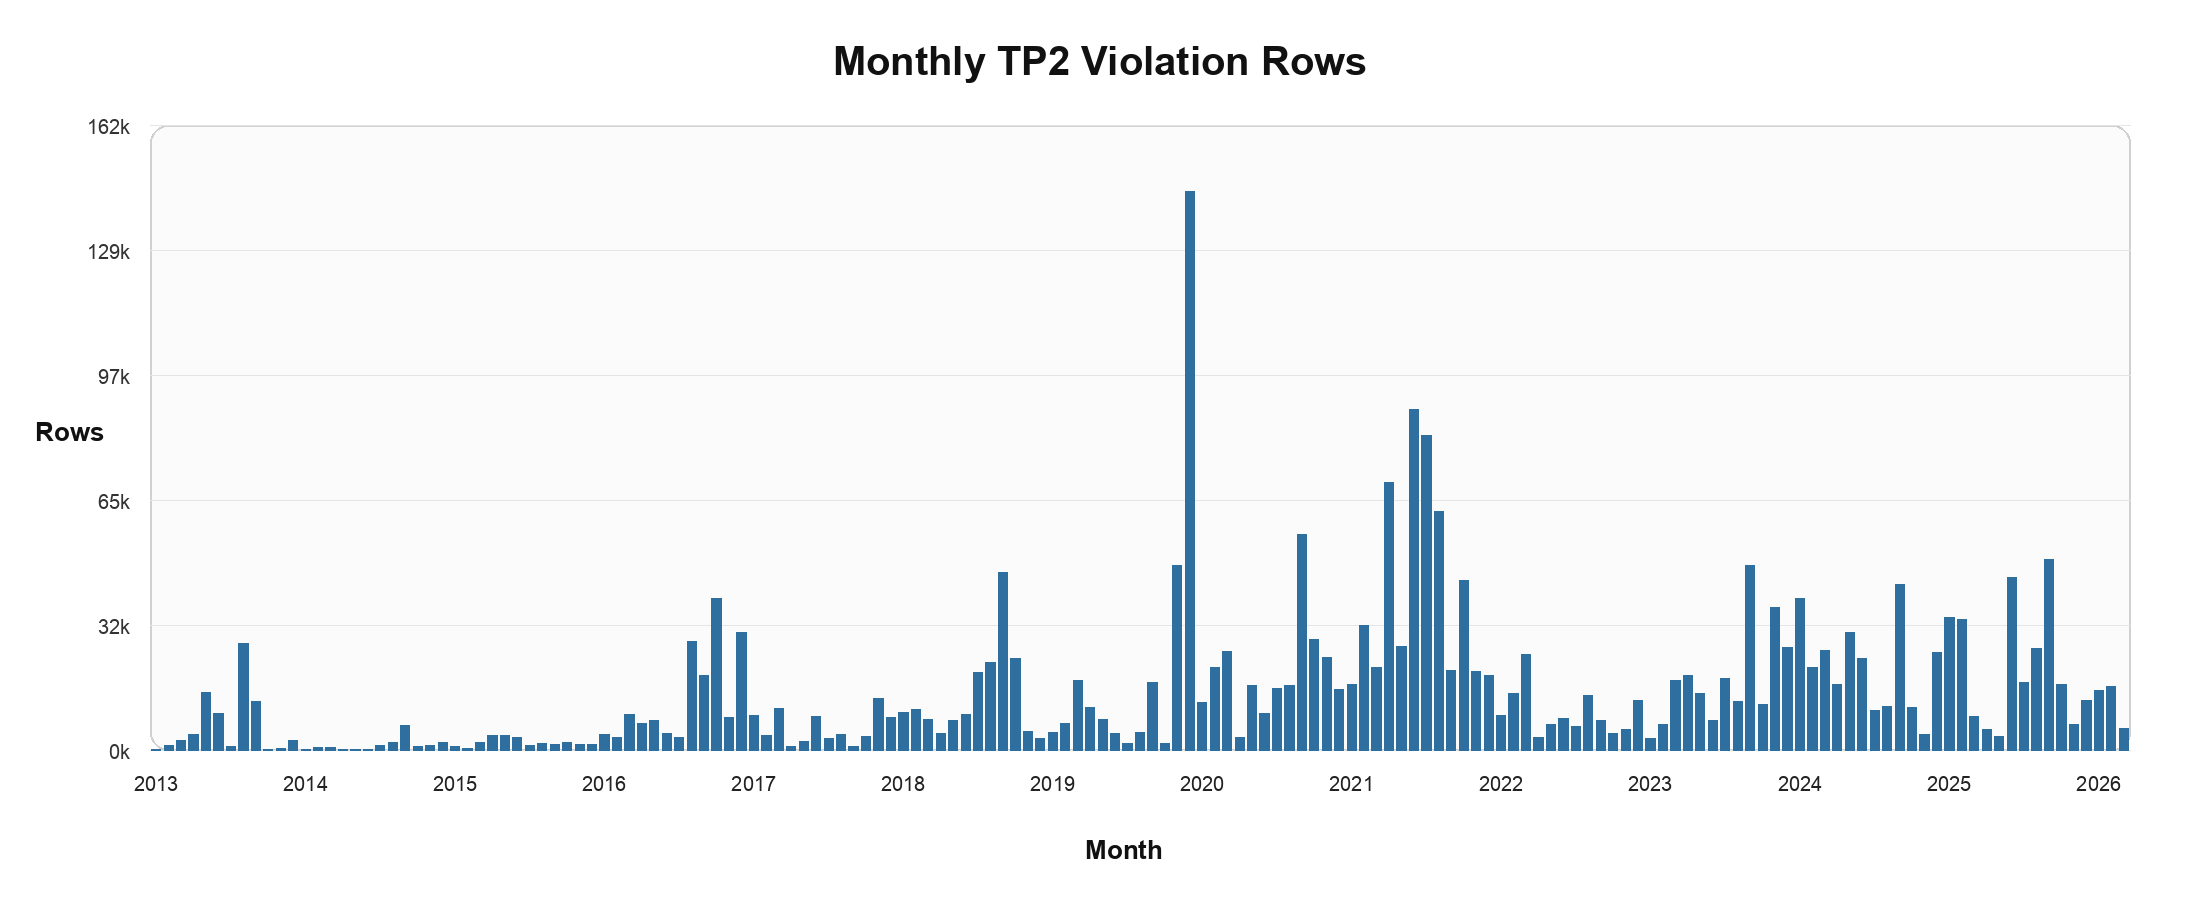
\includegraphics[width=0.96\textwidth]{raw_archive2_eda/figures/lastquote_tp2_violations_by_month.png}
\end{center}

\section*{Current Caveats}

\textbf{What I would say:}

There are three main caveats at this stage.

\begin{enumerate}
\item These counts are daily rectangle-level violations, not unique economic
episodes. The same rectangle can violate on adjacent days, so the next pipeline
must track episodes.
\item These are detector counts, not selected ML trades. We still need labels,
rolling-window ML, and a backtest with transaction costs and liquidity rules.
\item The clean dataset uses latest available quotes, not a guaranteed exact
3:59 or official close snapshot. This is acceptable for a research dataset if
we disclose it clearly and keep quote-quality filters strict.
\end{enumerate}

\section*{Next Pipeline Step}

\textbf{What I would say:}

The next technical step is episode tracking. Instead of treating every daily
violation row independently, we should create a stable rectangle key and group
the same violation across consecutive trading days into one episode. Then the
model should learn from episode starts, not from repeated daily observations of
the same event.

After episode tracking, we can rebuild labels and train the rolling-window ML
pipeline. That will make the research stronger because it avoids inflated
sample counts and gives a cleaner economic interpretation: how often a TP2
violation appears, how long it persists, whether it reverts, and whether a
trading rule can profit after realistic costs.

\section*{Closing Summary}

\textbf{What I would say:}

The dataset is usable and large enough for a publishable research pipeline, but
the raw EDA shows why transparent cleaning and episode construction are
necessary. We now have a validated full TP2 scan on the active cleaned data.
The next milestone is to convert daily violation rows into violation episodes,
then use those episodes for labeling, ML selection, and backtesting.

\end{document}
